%%%%%%%%%%%%%%%%%%%%%%% file template.tex %%%%%%%%%%%%%%%%%%%%%%%%%
%
% This is a general template file for the LaTeX package SVJour3
% for Springer journals.          Springer Heidelberg 2010/09/16
%
% Copy it to a new file with a new name and use it as the basis
% for your article. Delete % signs as needed.
%
% This template includes a few options for different layouts and
% content for various journals. Please consult a previous issue of
% your journal as needed.
%
%%%%%%%%%%%%%%%%%%%%%%%%%%%%%%%%%%%%%%%%%%%%%%%%%%%%%%%%%%%%%%%%%%%
%
% First comes an example EPS file -- just ignore it and
% proceed on the \documentclass line
% your LaTeX will extract the file if required
\begin{filecontents*}{example.eps}
%!PS-Adobe-3.0 EPSF-3.0
%%BoundingBox: 19 19 221 221
%%CreationDate: Mon Sep 29 1997
%%Creator: programmed by hand (JK)
%%EndComments
gsave
newpath
  20 20 moveto
  20 220 lineto
  220 220 lineto
  220 20 lineto
closepath
2 setlinewidth
gsave
  .4 setgray fill
grestore
stroke
grestore
\end{filecontents*}
%
\RequirePackage{fix-cm}
%
%\documentclass{svjour3}                     % onecolumn (standard format)
%\documentclass[smallcondensed]{svjour3}     % onecolumn (ditto)
\documentclass[smallextended]{svjour3}       % onecolumn (second format)
%\documentclass[twocolumn]{svjour3}          % twocolumn
%
\smartqed  % flush right qed marks, e.g. at end of proof
%
\usepackage{graphicx}
\usepackage{amsmath}
\usepackage{listings}
\usepackage{graphicx}
\usepackage{diagbox}
\usepackage{booktabs}
\usepackage{algorithm}
\usepackage{algorithmicx}
\usepackage{algpseudocode}
\usepackage{amssymb}
\usepackage[colorlinks,linkcolor=blue]{hyperref}
\usepackage{multirow}
%
% \usepackage{mathptmx}      % use Times fonts if available on your TeX system
%
% insert here the call for the packages your document requires
%\usepackage{latexsym}
% etc.
%
% please place your own definitions here and don't use \def but
% \newcommand{}{}
%
% Insert the name of "your journal" with
% \journalname{myjournal}
%
\begin{document}

\title{PatchID: An Overfitting Patches Identification Method for Automated Program Repair%\thanks{Grants or other notes
%about the article that should go on the front page should be
%placed here. General acknowledgments should be placed at the end of the article.}
}


%\titlerunning{Short form of title}        % if too long for running head

\author{Xuan Zhou         \and
        Xingqi Wang %etc.
}

%\authorrunning{Short form of author list} % if too long for running head

\institute{Xuan Zhou \at
              School of Computer Science, Hangzhou Dianzi University,Hangzhou, 310018, Zhejiang, China.\\
              Tel.: +86-19550151187\\
              %Fax: +123-45-678910\\
              \email{212050276@hdu.edu.cn}           %  \\
%             \emph{Present address:} of F. Author  %  if needed
           \and
           Xingqi Wang \at
              School of Computer Science, Hangzhou Dianzi University,Hangzhou, 310018, Zhejiang, China.\\
              \email{xqwang@hdu.edu.cn}
}

\date{Received: date / Accepted: date}
% The correct dates will be entered by the editor


\maketitle

\begin{abstract}
Automated Program Repair (APR) needs to verify the correctness of patches after they are generated. Typically, APR uses a test suite as the standard for patch correctness verification. However, the test suite is unable to fully represent the oracle of the program, which causes APR to generat a large number of overfitting patches that not only fail to fix the original error, but also cause new errors. To help developers identify overfitting patches, this paper proposes an overfitting patch identification method called PatchID. The core idea of PatchID is that the dynamic behavior of the passing tests between the buggy program and the correct patch is the same, however the dynamic behavior of the failing tests between them is different. The algorithm first constructs the dynamic behavior expressions that cause the bug from the program and the test suite, then generates new tests to enhance the original test suite, and finally gets the same dynamic behavior expressions from the patch, and identifies whether the patch is overfitting according to whether the value of the dynamic behavior expression changes with the use of the patch. The paper is evaluated on two datasets consisting of 155 Defects4J patches and 365 Java + JML patches, respectively. PatchID successfully identifies 93 overfitting patches and 9 correct patches on the first dataset, and 225 overfitting patches on the second dataset. In addition, PatchID classifies overfitting patches into three types of patches. Experiments show that the method proposed in this paper is superior to the existing similar methods.
\keywords{automatic program repair \and  overfitting patch \and program state
	abstract \and test generation}
% \PACS{PACS code1 \and PACS code2 \and more}

\end{abstract}

\section{Introduction}
\label{1}
Automated program repair (APR) has been widely studied in the past decade, leading to the emergence of many repair techniques. Among them, test-suite-based repair techniques are the most common, particularly since the proposal of GenProg\cite{ref1,ref2,ref3}. The test-suite-based APR takes a given test suite as oracle and generates patches that are considered correct if they passes the test suite. Accurally, the test suite is weak and can not fully represent the oracle of the program, which results in the existence of patches that pass all the tests but are still wrong, that is, overfitting patches. As a result, APR technology produces a large number of invalid patches. Current APR technologies are far from mature, and most of them will simply accept patches that pass the test suite . Therefore, further research and improvement of repair techniques are needed to improve the quality and accuracy of patches. According to Xin\cite{ref4}, a majority of patches generated by GenProg, AE, and RSRepair are incorrect. Recent research has focused on alternative repair methods, such as using human-written patches, repair templates and condition synthesis, bug-fixing instances  and forbidden modifications. However, these methods still face challenges in terms of low repair performance.

Due to the poor performance of repair techniques, developers have to manually verify a large amount of  overfitting patches, which consumes a lot of resources. Therefore, it has become an urgent problem to identify overfitting patches . Overfitting patch identification  methods typically follow this approach: after the APR tool generates patches, these patches are identified and overfitting patches are excluded, thus avoiding overfitting problems. However, those methods have problems such as low accuracy and limited additional information provided in the results. This results in developers still having to manually detect a large number of overfitting patches, so there is no significant improvement in the speed of fixing bugs. To solve these problems, further research and improvement of overfitting patch identification is needed.

Currently, being able to identify whether a patch is overfitting is already a successful achievement. Fast detection of overfitting patches can speed up the process of developers fixing errors. However, if a technique can classify overfitting patches, it can provide additional information to developers and further improve the speed of fixing the bug. According to Yu\cite{ref5}, overfitting patches can be classified into the following three categories:

\begin{itemize}
	\item[$\bullet$] A-Overfitting Patch: The patch does not completely fix the incorrect behavior nor does it destroy the original correct behavior.
	\item[$\bullet$] B-Overfitting Patch: The patch that fixes the original incorrect behavior but destroys the original correct behavior, which is also called regression.
	\item[$\bullet$] AB-Overfitting Patch: The patch destroys the original correct behavior instead of fixing the incorrect behavior.
\end{itemize}

Because the test suite is not complete, it is far from sufficient to  use the consistency of the actual output of the program and the test output, that is to say, the current APR does not take full advantage of the test suite, only uses the input and the output of the test suite, and does not dig into the hidden information in the test suite. At present, different overfitting identification methods have been proposed. Among them, Xiong et al. \cite{ref6} proposed a technology to explore the deep behavior of the test suite and program. By using the idea of TEST-SIM and PATCH-SIM, they were able to successfully exclude some overfitting patches, achieving a success rate of 56$\%$. In addition, experiments by Yang et al. \cite{ref7} showed that patches can change program behavior. They attempted to describe program behavior using program invariants, observing the expected behavior of the program from another perspective. These studies inspired us to propose a new technology for addressing overfitting issues - PatchID.

The goal of PatchID is to determine the category of a patch by digging into the correct behavior of the program based on a given test suite. While patches are able to pass the test suite, the passing tests reflect the correct behavior of the program, and the failing test reflect the wrong behavior of the program. From this point of view, patches should maintain the correct behavior of the program and modify the wrong behavior of the program. We believe that there are specific relationships between variables in a correct program, which are reflected by their values at runtime, and these relationships are a manifestation of the correct behavior of the program. So PatchID identifies a patch based on the following two important observations, which are from the perspective of program runtime variables:

\begin{itemize}
	\item[$\bullet$] PATCH-SIM: After using the patch, the dynamic behavior of the program of the passing test (the specific relationship between variables is represented in 5-tuples in this article, called snapshot) is similar to that before, while the dynamic behavior of the program of the failing test is different.
	\item[$\bullet$] TEST-SIM: When two tests have the same dynamic behavior, the two tests belong to the same category, that is, they belong to either the passing test or the failing test.
\end{itemize}

Based on the above two points, this paper designs and implements PatchID, and verifies the method on a dataset consisting of 155 patches.These patches were generated by APR technology based on Defects4J, including HDRepair\cite{ref17} , jGenprog\cite{ref8}, ACS\cite{ref9}, jKail\cite{ref10}, and Nopol\cite{ref11}. Our method successfully identified 93 overfitting patches and 9 correct patches out of these 155 patches. In addition, PatchID further classified the 93 overfitting patches into three categories, which is currently not available in other technologies. We also validated our method on a dataset of 365 Java + JML patches\cite{ref54}, and successfully identified 225 patches.

In summary, the paper makes the following main contributions :

\begin{itemize}
	\item[$\bullet$] Proposed a program state abstraction representation for calculating program execution similarity.
	\item[$\bullet$] Designed an overfitting patch identification and categorization algorithm.
	\item[$\bullet$] A framework for overfitting patch identification was implemented and evaluated. The results show that the framework is effective.
\end{itemize}

The rest of the paper is organized as follows. Section 2 first discusses related work. Section 3 describes some necessary concepts involved in our method. Section 4 introduces our approach in details. Section 5 describes our evaluation on two datasets. Section 6 discusses the threats to validity. Finally, Section 7 concludes the paper.

\section{Related work}
\label{2}

\subsection{Automatic Program Repair}
\label{2.1}
Generally, automatic program repair includes three steps: fault location, patch generation and patch verification. They will first generate some candidate patches, then use the existing test suite to verify these candidate patches, and the candidate patches that pass the test suite will be regarded as the correct patches. At present, the existing methods can be roughly divided into the following three categories: 

\begin{itemize}
	\item[$\bullet$] Heuristic Search-Based APR: Heuristic search-based automatic repair technology generates the repair patch by artificially defined heuristic rules. This kind of algorithms inlcude GenProg, ARJA-e \cite{ref12,ref13,ref14,ref15}, PraPR\cite{ref16}, etc, which use genetic algorithm to generate patches with the original program as search space. In addition, there are approaches, such as HistoricalFix\cite{ref17}, CapGen \cite{ref18}, ConFix\cite{ref19} to generate patches from historical repair patches and those as SCRepair\cite{ref20}, CRSearcher\cite{ref21}, SSFix \cite{ref22}, SimFix\cite{ref23}, Refactory\cite{ref24} to generate patches bycode similarity.
	\item[$\bullet$] Template-Based APR: It generates patches based on manual template. According to the experience of developers or researchers, some patch templates or patch generation strategies are predefined to guide the repair process. PAR\cite{ref25},iFixR\cite{ref26},SapFix\cite{ref27},ErrDoc\cite{ref28},BovInspector\cite{ref29}, LeakFix\cite{ref30}, AutoFix\cite{ref31}, GumTree\cite{ref32}, SketchFix\cite{ref33}, NPEfix\cite{ref34},F1X\cite{ref35}, HERCULES\cite{ref36}, and the anti-pattern method proposed by Tan\cite{ref37} fall into this category of algorithms.
	\item[$\bullet$] Semantic Constraint-Based APR: Semantic Constraint-Based APR infers the correct specification of the program by some means as a constraint to guide the patch generation or to verify the correctness of the patch.SemFix\cite{ref38}, DirectFix\cite{ref39}, Angelix\cite{ref40}, AllRepair\cite{ref41}, Nopol,S3\cite{ref42}, SemGraft\cite{ref43}, MemFix\cite{ref44}, FootPatch\cite{ref45}, SearchRepair\cite{ref46}, SOSRepair\cite{ref47} belong to this kind of algorithms.
\end{itemize}

All these repair techniques use G$\And$V method to produce patches. For these technologies, if a patch passes the test suite, it is the correct patch. However, a program cannot be fully tested, and the test suites given by existing datasets are all weak\cite{ref10}, so repair techniques will always produce a large number of overfitting patches on these datasets. New techniques are needed to find to identify these overfitting patches.

\subsection{Detection Of Overfitting Patches}
\label{2.2}
Currently, there are numerous techniques proposed and implemented for detecting overfitting patches, which can be classified into the following two categories:
\\ \hspace*{\fill} \\
\textbf{1. Oracle-based completion method}
\\ \hspace*{\fill} \\
As the test suite is unable to fully express the program’s oracle, two methods are available to complete the oracle in order to identify overfitting patches.

Xin et al. proposed DiffTGen \cite{ref49}, which attempts to address overfitting in APR by generating new test cases and using semantic differential checking between the buggy program and patch. The generated test cases are then added to the existing test suite to enhance it. In 2018, Mechtaev et al. proposed SemGraft \cite{ref50} to tackle the overfitting problem. They introduced a reference program as an oracle, which has the same functionality as the buggy program but is implemented differently. This method transforms the detection of overfitting patches into a semantic difference problem, using the semantic symbol abstract of the reference program as an oracle, to identify overfitting patches.
\\ \hspace*{\fill} \\
\textbf{2. Patch Filtering}
\paragraph{Patch Ranking.} Patch Ranking. Usually, APR can generate multiple candidate patches for a single bug. This method can rank these candidate patches, with higher-ranked patches being considered correct and lower-ranked ones being considered overfitting. Fan et al. \cite{ref51} learned a patch identification model through studying manually repaired patches, using this model to rank candidate patches and exclude those with lower rankings.
\paragraph{Patch Identification.}  This method directly provides the type of a candidate patch and does not use a ranking method to filter patches. Tan et al. \cite{ref52} extracted anti-patterns from APR patches to exclude those containing illegal repairs. Cashin et al. \cite{ref53} proposed PATCHPART, which tries to find program invariants in the buggy program to validate whether the patch violates program invariants and exclude overfitting patches. Nilizadeh \cite{ref54} validated the effectiveness of APR techniques using JML as an oracle on small programs, but JML is ineffective for large projects such as Defects4J. Xiong et al.\cite{ref6} introduced PATCH-SIM and TEST-SIM, which do not require an oracle and heuristically classify new generated test cases (input data) based on similarity of program execution paths to detect patches. This method is stringent in detecting overfitting patches based on path similarity, but does not further classify them. Ghanbari et al. \cite{ref55} proposed ObjSim, which compares system states before and after using a patch at the exit point of the patch method, and uses a similar idea to PATCH-SIM to identify overfitting patches. Ye et al. \cite{ref56} introduced ODS, a deep learning-based overfitting identification tool that extracts 202 code features for each patch, encodes them, and then uses a decision tree-based ensemble learning model to determine whether a patch is overfitting.

\section{PRELIMINARIES}\label{3}
To identify whether a patch is overfitting, PatchID relies on the following basic concepts.
\subsection{Program State Abstraction}\label{3.1}
In order to describe the dynamic behavior of a program at runtime, this paper introduces the concept of program state abstraction \cite{ref57}. Program state abstraction is composed of program variables, basic expressions, extended expressions, and boolean expressions. These expressions are collectively referred to as dynamic behavior expressions.

\textbf{Variables.} During the execution of each test, the values of these program variables are added into the set $ M_{\ell}$. These program variables are derived from two types of data.
\begin{itemize}
	\item[$\bullet$] Exact values of numeric and boolean types
	\item[$\bullet$] Object identifier for a reference type expression
\end{itemize}

\textbf{Expressions.} In a program, reference types or numeric types can be monitored. These type of variables make up the basic expressions, which include 
(1) local variables (including parameters of $M_{bug}$) declared inside $M_{bug}$ (the method where the bug occurs), and these variables are visible at $\ell$; (2) attributes of the class to which the $M_{bug}$ belongs; (3)Any expression that can be evaluated at $\ell$, but expressions with side effects such as increment, decrement, assignment, and creation cannot be monitored. In this paper, we use $E_{\ell}$ to denote the set of all monitorable basic expressions at $\ell$ ($\ell$ denotes the unique identifier of each statement). For each reference type $r$ in the $E_{\ell}$, the following two forms form the extended expression, including: (1) $r.f()$, $f()$ is a no-argument function and returns a type that can be monitored at $\ell$. (2) When $r$ is this, the attributes of $r$ are monitorable at $\ell$. In this paper, we use $X_{\ell}$ to denote the set of all extended expressions that can be monitored.

In order to explain the expression in detail, Figure \ref{fig1} and Figure \ref{fig2} show the buggy program and its corresponding patch, Figure \ref{fig3} and Figure \ref{fig4} show the passing test and the failing test, respectively. The buggy program functions as follows: The duplicate method receives two ArrayLists $(list1,list2)$ and an int $n$. Its function is to copy $n$ elements from $list2$ to $list1$.However, this program has an obvious error, which ignores the case that $n$ is greater than the length of $list2$, When $n$ is greater than the number of elements of $list2$, the program will throw Index Out Of Bounds exception. $if$ statement is appended into the patch to avoid this error. $count$ in the first line of the buggy program, $list1$, $list2$, and $n$ in the arguments, are all basic expressions that can be monitored. At this point, the extended expressions for $\ell$ are $list1.size()$, $list2.size()$, and so on.
% For one-column wide figures use
\begin{figure}[htbp]
	\centering
	\begin{minipage}[t]{1\textwidth}
		\centering
		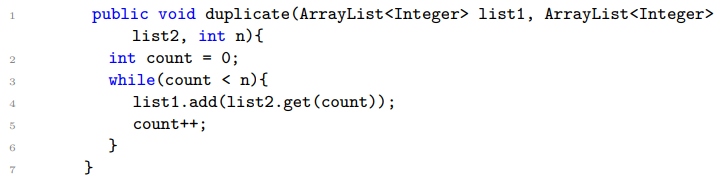
\includegraphics[width=1\textwidth]{fig1.png}
		\caption{Buggy program}\label{fig1}
		\vspace{5mm}
	\end{minipage}
	
	\begin{minipage}[t]{1\textwidth}
		\centering
		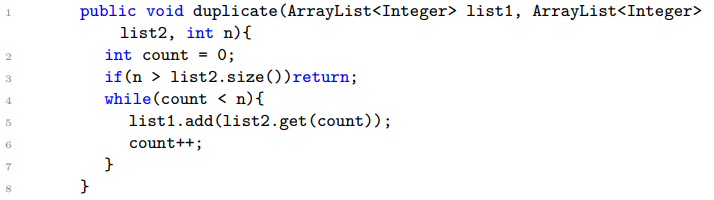
\includegraphics[width=1\textwidth]{fig2.png}
		\caption{Patch}\label{fig2}
		\vspace{5mm}
	\end{minipage}
	
	\begin{minipage}[t]{0.5\textwidth}
		\centering
		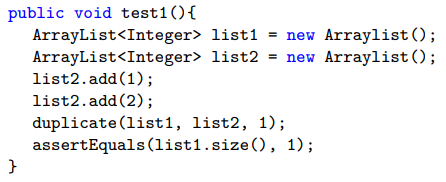
\includegraphics[width=1\textwidth]{fig3.png}
		\caption{Passing test: test1}\label{fig3}
	\end{minipage}
	\begin{minipage}[t]{0.48\textwidth}
		\centering
		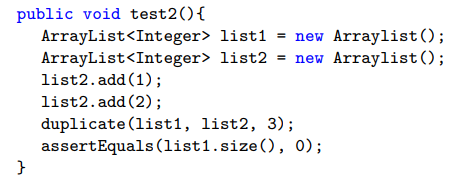
\includegraphics[width=1\textwidth]{fig4.png}
		\caption{Failing test: test2}\label{fig4}
	\end{minipage}
\end{figure}

\textbf{Boolean expressions.} Boolean expressions are composed of relational expressions and logical expressions. In this paper, we denote by $B_\ell$ a boolean abstract set at $\ell$. Boolean expressions can be expressed in the following four forms: (1)for each pair $k_1,k_2 \in E_\ell \cup X_\ell$ of expressions of the same type, $B_\ell$ includes $m_1 == m_2$ and $m_1 \neq m_2$; (2)for each pair $k1,k2 \in E_\ell \cup X_\ell$ of expressions of integer type, $B_\ell$ includes $k_1 \bowtie k_2$,for $ \bowtie \in \{ <,>,\leq,\ge \}$; (3)for each expression $b \in E_\ell \cup X_\ell$ of boolean type,$B_\ell$ includes $b$ and $!b$; (4)for each pair $b_1,b_2 \in E_\ell \cup X_\ell$ of expressions of boolean type, $B_\ell$ includes $b_1 \vee b_2$ and $b_1\wedge b_2$.

For example, in the first line of Figure \ref{fig1}, $n$ and $list2.size()$ are both monitorable expressions, and both are of the same Integer type. Then the following six boolean expressions can be composed:  $n>list2.size(), n>=list2.size(), n<list2.size(), n<=list2.size(), n==list2.size(), n!=list2.size()$.The boolean expression $n>list2.size()$ causes the program error. If the test satisfies this boolean expression, when the program enters the $while$ loop, $count$ will eventually equal $list2.size()$, which causes the program to throw an out-of-range error. So this results in test1 being a passing test and test2 being a failing test, because the size of $list2$ in test2 is less than 3.

\subsection{PATCH-SIM and TEST-SIM} \label{3.2}
As mentioned earlier, a test suite is not like a formal specification in that its coding specifications are weak and incomplete. Low-quality test suites are a key reason why APR generates overfitting patches. To take full advantage of existing and enhanced test suites for filtering overfitting patches, we need the following two definitions:

\begin{definition}[TEST-SIM]
	When two tests have the same program behavior, then they will have the same test result, that is, the boolean expression b and the corresponding value are the same at the same statement, then both tests should be either a passing test or a failing test.  
\end{definition}
APR usually takes the patch that passes all tests as the correct patch, but the test suite cannot express a complete oracle. To enhance the test suite, we need to generate new tests, but PatchID's method of generating new tests does not and cannot know what the test output is. Only boolean expressions at run time are available. For example, there is a new test with $list1.size = 0$, $list 2.size = 5$, and $n = 10$. Then the boolean expression of the test in the third line of the buggy program in Figure~\ref{fig1} is $n > = list2.size(),true$, which is the same as the boolean expression of test2 at this point, so this test is considered to be a failing test.
\begin{definition}[PATCH-SIM.]
	With the correct patch, the passing test is the same as the previous boolean expression and its value, while the failing test should be different. 
\end{definition}
For example, in a buggy program, all passing tests result in a boolean expression $b$ being false, and all failing tests result in $b$ being $true$.Then determining whether the patch is overfitting is not just a single way to observe the output of the program, but by comparing the value of $b$ in a statement before and after using the patch. The value of $b$ should be consistent with the buggy program when the patch runs the passing test; it should be different from the buggy program when the patch runs the failing test. According to PATCH-SIM, we can see that in the previous example, patch is correct, because in the fourth line (corresponding to the third line of the buggy program), $n > list 2.size()$ no longer exists, and all tests that make this boolean expression true will go to the $return$ statement.

Through these two observations, we can dig out more information from a buggy program and a test suite, so that the identification of patches does not need oracle. New tests are heuristically classified by TEST-SIM, and patches are heuristically classified by PATCH-SIM.

\section{APPROACH}\label{4}
This section mainly introduces the detailed process of PatchID, including its overview and three main modules, i.e. Snapshot finder, Test generation, and Identification.

\subsection{Overview}\label{4.1}
Figure \ref{fig5} below shows the overall flow of our approach.

\begin{figure}[ht]%
	\centering
	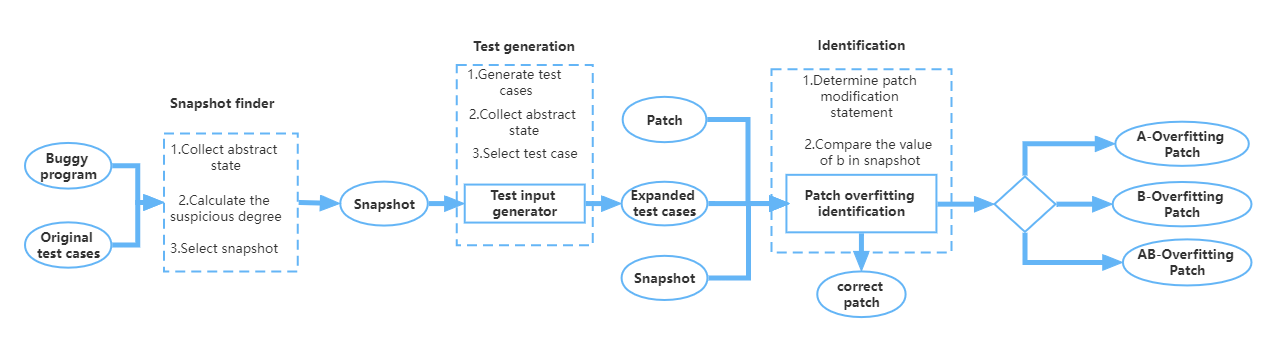
\includegraphics[width=1\textwidth]{fig5.png}
	\caption{Approach Overview}\label{fig5}
\end{figure}

Take a buggy program, an original test set $t_o$, and the corresponding patch as input. This method firstly find the most suspicious snapshot $s$ through Snapshot finder, and then generate new tests through $s$ and Test input generator. Secondly, the new tests are added to the test suite to generate the extended test suite $t_e$. PatchID runs patches with $t_e$ and saves the values of the expressions in $s$. Finally, PatchID indentifies a overfitting patch by observing whether the expression value of each test case changes before and after using the patch. And the overfitting patches are subdivided further.

\subsection{Snapshot Finder}\label{4.2}
Snapshot finder is designed to find the most suspicious snapshot $s$. This step has two functions. One is to provide a standard for generating new tests in the next step, so as to classify the new tests; the other is to compare the snapshot set obtained after running the test set for the patch in the third step in order to identify the type of the overfitting patch.

\textbf{snapshot.} snapshot $s$ can be expressed as a 5-tuple $s= \langle \ell,b,?,i,v_i \rangle$,where $\ell$ is the unique identifier of each statement, $b$ is a boolean expression, $?$ is the value of $b$ (true or false), $i$ represents the unique serial number of each test in the test suite, and $v_i$ represents the actual value of $b$ of the test $t_i$ during $M_{bug}$ execution. Each snapshot has a corresponding suspiciousness value. The suspiciousness of a snapshot is used to measure the likelihood of a bug.The snapshot with the maximum suspiciousness is most likely to cause a bug in the program.The suspiciousness is determined by the following two factors: (1)a syntactic analysis of expression dependence $ed_s$; (2)a dynamic analysis $dy_s$. $ed_s$ increases as the number of occurrences of $b$ before and after $\ell$; The more times $?$ corresponding $b$ appears in failing tests and the less times $?$ corresponding $b$ appears in passing tests, the greater the value of $dy_s$. The formula\cite{ref57} for calculating the degree of suspicion in this paper is defined as follows:
\begin{equation}
	2/({ed_s^{-1}}+dy_s^{-1})
\end{equation}
Because of the limitation of formula above for calculating the degree of suspicion, $?$ is not exactly the same as the result $v$ of the actual execution of the test, so we must note that $?$ is used to classify new tests and $v$ is used to classify patches. Snapshot is the core of this algorithm. This paper designs the following algorithm to construct Snapshot.
\begin{algorithm}
	\caption{get the most suspicious snapshot}\label{algo1}
	\begin{algorithmic}[1] 
		%\Require Input
		%\Ensure Output
		\Require
		$t_o$: original test suite;
		$M_{bug}$
		\Ensure
		optimal $s_{bug}$
		\State $ex_b \gets null$
		\Function {"getSnapshot"}{}
		
		\State $ex_b$ = createBooleanExpression($M_{bug}$);
		
		
		%for
		\For{$i = 0$; $i < n$; $i++$}
		%
		
		\If {coverBugM($t_i$)} \State  compute($ex_b$) \State
		buildSnapshot($ex_b,t_i$)
		\Else \State delete($t_i$);
		\EndIf
		\EndFor
		\State
		calculateSuspiciousness()
		\State $s_{bug}$ = getSnapshot();
		
		\Return $s_{bug}$
		\EndFunction
		
	\end{algorithmic}
\end{algorithm}

In the first step of this algorithm, PatchID creates a boolean expression set for each statement $\ell$. Secondly PatchID uses $t_o$ to run the buggy program, then saves the program abstraction state in the tests that cover $M_{bug}$, calculates the value of each boolean expression in the set (real value $v$) and build the snapshot. If $t_i$ does not cover $M_{bug}$, this test is deleted. The third step is to calculate the suspicious degree of each snapshot. At this time, $?$ is obtained(PatchID will use this value to generate new tests). The fourth step is to select the most suspicious snapshot $s$. If there are multiple snapshots, select one of them at random. For the subsequent process, PatchID will save a snapshot set $s_{bug}$, $\ell$,$b$,$?$ as with $s$, $i$ and $v$ holds the real value for each test. In the previous example, $s= \langle 3,n>=list2.size(),true,i,v \rangle$ represents the boolean expression $n>=list2.size()$ in the third line of the buggy program, the error occurs because expression is evaluated to be true.
\subsection{Test Generation}\label{4.3}
The goal of Test generation is to generate new tests using the TEST-SIM criterion. PatchID does not need to care about whether the output of these tests is correct, but it needs to know the value of the boolean expression $b$ in the snapshot generated by these tests to be the same as $?$ of $s$. This means that PatchID requires some new failing tests that are used to enhance the test suite.

PatchID uses Evosuite\cite{ref58}, an existing automated test generation tool, to generate a set of tests. Because Evosuite generates test cases for a class, the test cases should be selected. Similar to the steps in the Snapshot finder, select the test that covers the $M_{bug}$ and save the program abstract state and snapshot. If the snapshot$(\ell,b,v)$ of the new test corresponds to the most suspicious $s(\ell,b,?)$ respectively, then new failing tests will be added to the test suite $t_e$. PatchID does not select the new passing tests, because for the passing tests, $M_{bug}$ not only outputs correctly, but also behaves correctly.

\subsection{Identification}\label{4.4}
The purpose of this step is to determine if a patch is overfitting. It requires that snapshot set $s_{bug}$, extended test suite $t_e$, and the patch are provided previously. PatchID will run patch with the extended test suite, save the snapshot set $s_{patch}$, and then compare it with $s_{bug}$ to determine the type of patch.

\subsubsection{Select Statement}\label{4.4.1}

For buggy programs, patches typically include the following operations, that is, insert, delete, replace, and update. Then the $\ell$ in the snapshot of the buggy program cannot be directly monitored in the patch, because the position of the statement has changed, and the statement $\ell_{patch}$ in the patch needs to be relocalized to monitor the same boolean expression $b$. We believe that no matter what kind of repair operation, the program can have correct program behavior only after the repair operation is completed, so the method in this paper selects the position of $\ell_{patch}$ in the next statement after the modification is completed. For some special cases, we also need to use other rules.
We denote $start_s$ as the first statement that differs between the buggy program and the patch, and $end_s$ as the last statement that differs. The rules for localizing $start_s$ and $end_s$ are defined as follows:
\begin{itemize}
	\item[$\bullet$] If $start_s$ is a block statement such as $for, while, if$, etc. and $end_s$ is inside this block statement, then $\ell_{patch}$ is the next statement at the end of the  block.
	\item[$\bullet$] If $start_s$ and $end_s$ lie in sequential statements, $\ell_{patch}$ is the next statement in $end_s$.
	\item[$\bullet$] If $end_s$ is the last statement of a program or a block of code, $\ell_{patch}$ = $end_s$
\end{itemize}

\subsubsection{Patch identification}\label{4.4.2}
After $\ell_{patch}$ is determined, PatchID will run patch using the test suite $t_e$ to obtain the snapshot set $s_{patch}= \{ \langle \ell_{patch},b,?,i,v_i \rangle \mid i=0,1,\dots,n \}$. The steps for obtaining $s_{patch}$ are similar to those in 4.2. The next step is to compare two snapshot sets $s_{bug}$ and $s_{patch}$ to determine whether the patch is overfitting.It is worth noting that overfitting patch classification is also performed concurrently, as when a candidate patch is identified as an overfitting patch, it will be further classified.

In order to identify overfitting patches, two variables $N_f$ and $N_p$ are needed to be calculated. For a failing test, $N_f$ represents the number of same value of $v$ between the two sets. For a passing test, $N_p$ represents the number of different value of $v$ between the two sets. Given the values of the variables $N_f$ and $N_p$, the type of patch is defined as follows:
\begin{equation}
	detection(p)= \begin{cases} A& N_f>0\bigwedge N_p = 0\\ B& N_f=0\bigwedge N_p>0\\
		AB& N_f>0\bigwedge N_p>0\\ correct& N_f = N_p = 0\end{cases}
\end{equation}
We map two snapshot sets one by one according to the unique identifier $i$ of the test, and compare the $v_i$ values of each test before and after using the patch. Depending on the type and source of tests, $t_e$ is divided into three categories, that is passing, failing, and new. If $t_i \in t_{passing}$, $N_p++$ when $v_i$ is different; if $t_i \in t_{failing} \cup t_{new}$, $N_f++$ when $v_i$ is the same. After the two sets are compared, the values of $N_f$ and $N_p$ can be obtained. The type of the patch can be determined according to the above formula, $N_f$ and $N_p$.
For example, $v$ corresponding to tese1 and test2 in the buggy program is false and true respectively. And both of their values in patch are false. Then $N_f = N_p = 0$, and patch is treated as correct.

\section{EVALUATION}\label{5}
 To experimentally evaluate the effectiveness of the PatchID, we propose the following four research questions:
\begin{itemize}
	\item[$\bullet$] RQ1: How effective is PatchID in identifying overfitting patches? Does it have any advantages over other methods?
	\item[$\bullet$] RQ2: How efficient is PatchID while identifing patches?
	\item[$\bullet$] RQ3: What causes errors in identifying overfitting patches?
	\item[$\bullet$] RQ4: How reliable is PatchID for overfitting patch classification?
\end{itemize}
\subsection{Dataset}\label{5.1}
The article evaluated PatchID on two datasets. The first dataset was collected in the study of Xiong et al. \cite{ref8}, consisting of patches generated by six APR tools on Defects4J. It is worth noting that, to conduct comparative experiments, we used the same Defects4j dataset as used in Xiong's study, but we did not run any APR tools to collect patches. The patch identification results have already been provided by the APR authors. The second dataset, Java+JML, was created by Nilizadeh et al., and the patch results were provided by the original authors. We compared the results presented by PatchID with the results provided in the datasets to evaluate its efficacy.

\textbf{Defects4J.} At present, Defecets4j proposed by Just\cite{ref59} is the most widely used Java program dataset in the field of automatic program repair. Defects4J has 17 projects so far, which contain 835 defects. Each program defect in this dataset contains at least one test that can trigger it.This paper uses the six most frequently used projects in the dataset, namely, Chart, Time, Math, Lang, Closure and Mockito, where Chart is a project dedicated to displaying icons, Time is a project used for date and time processing, Math is a project for scientific computing, and Math is a project for displaying icons; Lang is a set of additional methods for manipulating JDK classes; Closure is an optimizing compiler for Javascript; Mockito is a mock framework for unit testing.

According to the information provided by Xiong, the candidate patches were generated by six APR tools. The six APRs are jGenProg, Nopol 2015, Nopol 2017, ACS, HDRepair and jKali, respectively. jGenProg is the Java version of GenProg, which is a heuristic search repair tool based on genetic algorithm. Nopol is a technique for fixing conditional statement errors in Java programs. It gives different repair strategies according to the type of error statement. If the location of the error code is a conditional statement, Nopol usually generates a repair patch to modify the original conditional statement; if the location of the error code is a non-conditional statement, it simply adds a new condition to skip the execution of the current statement. This paper includes two versions of Nopol 2015 and Nopol 2017. ACS is a conditional statement synthesis tool with high precisiton, which extracts patch templates for repair based on statistical analysis. HDRepair is also a repair tool based on statistical analysis. JKali is a re-implementation of Kali on Java, which is a repair tool to remove buggy statement only.

There are a total of 220 patches in the dataset. In this paper, we experimented on these 220 patches to determine whether they are overfitting patches, and obtained the results of 165 patches in total.Among these 165 patches, except for 9 patches (because the classification of 9 patches was not given in the original dataset), the remaining 155 patches were determined as overfitting patches.Table \ref{tab1} gives the specific information of the 155 patches.
\begin{table}[ht]
	\begin{center}
		\begin{minipage}{\textwidth}
			\caption{Defects4j Dataset}\label{tab1}%
			
			\begin{tabular}{cccccccc}
				\toprule
				\diagbox{Project}{Tools} &Chart	&Closure	&Lang	&Math &Mockito &Time &Total \\ \hline
				Nopol  &12 &39	&10  &25 &1 &8 &96\\ 
				jKai  &5 &0	&0  &8 &0 &1 &14\\ 
				jGenprog  &6 &0	&0  &12 &0 &2 &20\\ 
				HDRepair  &0 &0	&2 &6  &0 &1 &9\\ 
				ACS  &1 &0	&4  &11 &0 &1 &17\\ 
				Total  &24 &39	&16  &62 &1 &13 &155 \\
				\bottomrule
			\end{tabular}
			
		\end{minipage}
	\end{center}
\end{table}

\textbf{Java+JML dataset.} The dataset proposed by Nilizadeh is the first validated and publicly available dataset for Java programs. It consists of the following four components: correct programs, mutated buggy programs, test suites, and APR-based patches. The programs in this dataset have JML specifications for experimental evaluation. This dataset implements various classical algorithms and data structures, such as bubble sort, factorial, queue, etc. They are small programs with formal specifications written in JML and, therefore, can be considered as programs with oracle. Test suites are created using AFL-based fuzzy tools. Test suites are divided into Small and Medium depending on the size of the number of generated test cases. Buggy programs are created using PITest, a Java program mutation tool that injects a single error into each java program.PITest generates errors by changing control conditions, changing assignment expressions, removing method calls, and changing return values. APR-based repair patches are obtained using the following repair tools, namely ARJA-E, Cardumen, jGenProg, jKali, jMutRepair, Kali-A, and Nopol.

We selected 236 overfitting patches based on Medium test suite and 336 overfitting patches based on Small test suite from the Java+JML dataset, which were judged by JML specification and determined that these patches were overfitting patches. The PatchID algorithm was run on a total of 572 patches, and the results were obtained for 365 patches, as shown in Table \ref{2}.
\begin{table}[ht]
	
		\begin{minipage}{175px}
			\caption{Java+JML Dataset}\label{tab2}%
			\begin{tabular}{ccc}
				\toprule
				PatchType & Collected & Validated \\
				\midrule
				Medium    &236 &144 \\
				Small    &336 &221 \\
				Total   &572 &365 \\
			\bottomrule
			\end{tabular}
		\end{minipage}
	
\end{table}
\subsection{Experiment Setup}\label{5.2}
We implemented PatchID on top of the JAID\cite{ref57} framework. we ran two datasets, the Defects dataset on Ubuntu 18.04, Defects4j 2.0.0, JDK1.8 and the Java+JML dataset on Windows 10, JDK1.8.

\textbf{RQ1.} To evaluate the effectiveness of PatchID, we ran the collected patch sets and saved the patch judgments and the values of important variables in a file. These variables are snapshot, passing test, failing test, and new test. In addition, we compared with two overfitting patch identification tools, PatchSim and ODS. PatchSim is a scheme proposed by Xiong, and we use the same criteria as his, namely PATCH-SIM and TEST-SIM, but he uses the program execution path perspective, while PatchID uses program dynamic expressions. To explore whether expression-based PATCH-SIM has better results relative to program path execution, so we choose Xiong's tool. ODS is an overfitting identification tool based on deep learning proposed by Ye \cite{ref56}. We chose ODS for comparison because it is the most recent overfitting patch identification tool and it works very well. We collected the results of ODS runs on the first dataset according to the manual given by the authors. We got 143 results, of which 9 patches are unknown and 95 patches are Ye's experiments that gave the results.  We took a concatenation operation of Ye's experimental results with 143 results, resulting in 163 patch identification results. We chose to compare on the first dataset because Defects4j is closer to the real project. It is worth noting that we chose 206 patches as the base (14 unknown types out of 220 patches) because the number of patch intersections supported by the three tools is too small.

\textbf{RQ2.} Record the running time of each patch, calculate the time in whole minutes, and approximate the extra seconds by rounding.

\textbf{RQ3.} Manually analyze misclassified patches and analyze the reasons for failure.

\textbf{RQ4.} In order to verify the effectiveness of PatchID on the classification of overfitting patches, we manually determined the specific classification of overfitting patches. Since the Defects4J program is too complex, this paper only analyzes it in the Java+JML dataset. The manual judgment is based on the different warnings generated from the warning file "ESC.txt" of the buggy program and the warning file "ESC\_Repaired.txt" of the patch in this dataset. These two warning files are provided by this dataset, and they are generated because when the state of a Java program at runtime does not conform to JML expectations, then a warning file is generated. The warning file records the lines in the program that do not conform to JML expectations, and records the corresponding JML statements. We compared each pair of warning files. When the number of warnings in ESC\_Repaired is less than that of ESC, we consider that the patch has not completely fixed the bug, i.e., A-overfitting patch; when new warnings appear in ESC\_Repaired, we consider that the patch introduces regression problems, i.e., B-overfitting patch; when both of these bugs exist, we consider the patch to be an AB-overfitting patch.

\subsection{Experimental Result}\label{5.3}
\subsubsection{Results of RQ1}\label{5.3.3}
\textbf{Performance on Defects4J.} Table \ref{tab3} and Table 4 show the results of PatchID runs on the APR tool and different projects, respectively. As shown in the table, PatchID successfully identifies 102 patches from 155 patches, including 93 over-fitted patches and 9 correct patches.
\begin{table}[ht]
		\begin{minipage}{\textwidth}
			\caption{Results By APR Tools}\label{tab3}%
			\begin{tabular}{ccccc}
				\toprule
				Tool & All-$\sharp$C & All-$\sharp$O &$\sharp$C  &$\sharp$O\\
				\midrule
				Nopol2015    &4 &20 &0 &10(50$\%$) \\
				Nopol2017    &3 &68 &1(33.33$\%$) &52(76.47$\%$)\\
				HDRepair    &4 &5 &3(75$\%$) &1(20$\%$) \\
				ACS    &11 &6 &4(36.36$\%$) &6(100$\%$)\\
				jKali    &0 &14 &0 &11(78.57$\%$)\\
				jGenprog    &5 &15 &1(20$\%$) &13(86.66$\%$)\\
				Total    &27 &128 &9(33.33$\%$) &93(72.65$\%$)\\
				\bottomrule
			\end{tabular}
			\footnotetext{"All-$\sharp$C/All-$\sharp$O"indicates the number of all Correct/Overfitting patches}
			\footnotetext{"$\sharp$C/$\sharp$O "indicates the number of Correct/Overfitting patches identified}
			
		\end{minipage}
\end{table}

\begin{table}[ht]
		\begin{minipage}{\textwidth}
			\caption{Results By Project}\label{tab4}%
			\begin{tabular}{ccccc}
				\toprule
				Tool & All-$\sharp$C & All-$\sharp$O &$\sharp$C  &$\sharp$O\\
				\midrule
				Lang    &6 &10 &2(33.33$\%$) &8(80$\%$) \\
				Math    &13 &49 &5(38.46$\%$) &34(69.39$\%$) \\
				Chart    &3 &21 &1(33.33$\%$) &12(57.14$\%$)\\
				Time    &2 &11 &5(50$\%$) &10(90.91$\%$) \\
				Closure    &2 &37 &0 &29(78.38$\%$)\\
				Mockito    &1 &0 &0 &0\\
				Total    &27 &128 &9(33.33$\%$) &93(72.65$\%$)\\
			\bottomrule
			\end{tabular}
		\end{minipage}
\end{table}
\textbf{Overfitting patch.}  From Table \ref{tab3}, we can find that PatchID works better on the five repair tools, Nopol 2015, Nopol 2017, jKali, jGenprog, and ACS (all can identify more than 50\% of overfitting patches), but it works worse on HDRepair (only 20\% of overfitting patches can be identified).

From Table \ref{tab4}, the effect of overfitting patch identification becomes more obvious. patchID performs the best in Time, identifying 90.91\% of overfitting patches. It performs the worst in Chart with only 57.14\%.

\textbf{Correct patch.} Among the 155 patches, there are 27 correct patches, and PatchID is able to identify 9 of them. Among them, the number of correct patches in Math is the largest, and PatchID identifies a total of 5.

\textbf{Performance on Java+JML dataset.} From the data in Table \ref{tab5}, it can be seen that PatchID can correctly determine 93 overfitting patches based on Medium type patches, identifying 64.58\% of overfitting patches; based on Small type patches, PatchID can determine 132 overfitting patches, identifying 59.73\% of overfitting patches.

It is clear from the accuracy rates of Medium and Small that the accuracy rate decreases as the number of test cases in the test suite decreases. This data shows that a weak test suite affects the PatchID judgment.

\begin{table}[ht]
		\begin{minipage}{175px}
			\caption{Results By PatchType}\label{tab5}%
			\begin{tabular}{ccc}
				\toprule
				PatchType & All-$\sharp$O & $\sharp$O\\
				\midrule
				Medium    &144 &93(64.58\%) \\
				Small    &221 &132(59.73\%) \\
				Total   &365 &225(61.64\%) \\
				\bottomrule
			\end{tabular}
		\end{minipage}
\end{table}

\textbf{Comparison with other tools.} We compared with other overfitting patch identification tools, and the experimental results showed that PatchID outperformed the other tools overall. As shown in Table \ref{6}, there are 170 overfitting patches and 36 correct patches out of 206 patches, among which PatchID identifies the most overfitting patches with 93. While ODS identifies 72 and PatchSim identifies 62. In terms of the number of correct patches identified, ODS identified the most patches with 26, PatchID identified 9, and PatchSim did not identify any of the correct patches. So overall, PatchID was able to correctly identify the most patches with 102, while ODS identified 98 and PatchSim only 62.

\begin{table}[ht]
	\begin{minipage}{175px}
		\caption{Comparison with PatchSim and ODS}\label{tab6}%
		\begin{tabular}{ccccccccc}
			\toprule
		\multicolumn{3}{c|}{Dataset} &\multicolumn{2}{c|}{PatchSim} 
		& \multicolumn{2}{c|}{ODS}
		&\multicolumn{2}{c}{PatchID}\\
		\toprule
		Project &$\sharp$O &$\sharp$C &$\sharp$O &$\sharp$C &$\sharp$O &$\sharp$C &$\sharp$O &$\sharp$C\\

		
			\midrule
			Chart	&23	&4	&13	&0	&14	&3	&12	&0  \\
			Closure	&54	&2	&0	&0	&0	&0	&29&	0\\
			Lang	&11	&6	&5	&0	&10	&6	&8	&2\\
			Math	&68	&21	&35	&0	&37	&16	&34	&5\\
			Mockito	&1	&1	&0	&0	&0	&0	&0	&1\\
			Time	&13	&2	&9	&0	&11	&1	&10	&1\\
			Total	&170	&36	&62	&0	&72	&26&	93	&9\\
			\bottomrule
		\end{tabular}
	\end{minipage}
\end{table}
\textbf{Answer to RQ1.} From the analysis of the experimental results, PatchID identifies overfitting patches well, and identifies 72.65\% and 61.64\% of overfitting patches on the two datasets, respectively. In addition, we compare with PatchSim and ODS on the Defects4j-based dataset. The results show that PatchID performs better than the first two in identifying overfitting patches. For the PatchSim, PatchID also uses PATCH-SIM and TEST-SIM, but PatchID identifies more overfitting patches and correct patches than the former, which indicates that the approach based on dynamic program behavior expressions applies PATCH-SIM and TEST-SIM better than the program execution path approach. It is worth noting that both ODS and PatchID have their own advantages; ODS is able to identify more correct patches and PatchID is able to identify more overfitting patches. However, when looking at the total number of patches identified by both, PatchID has the advantage, with 4 more than ODS. In general, PatchID is able to identify overfitting patches effectively, and is able to correctly identify more overfitting patches than other techniques of the same type under the same conditions.

\subsubsection{Results of RQ2}\label{5.3.2}
The goal of PatchID is to help developers determine overfitting patches more quickly and save time, so this paper focuses on the time spent by PatchID to determine a patch. We recorded the start time and end time of each patch from PatchID's logs, and finally got the running time of the patch.

\textbf{Performance on Defects4J.} We recorded the running time of 155 patches. As mentioned earlier, PatchID determines a patch in three steps, and the percentage of time spent on each step varies depending on the project. As shown in Table \ref{tab7}, most (57.42\%) of the patches got their results within 5 minutes. The second step, Test Generation, takes up most of the time during these patch operations, while the remaining time is spent on running the test cases and computing the Boolean expressions of the program. Patches that take more than five minutes to run take more time to obtain the program abstraction state, because our observation is that Evosuite usually spends 1 $\sim$ 2 minutes on Defects4J to generate new test cases. During the experiments in this paper, there were three patches that took more than 60 min to run, one of which took 123 min, the vast majority of which was spent running test cases. The average time to determine whether a patch is an overfitting patch is 11.6 min, of which 76.77\% are within the acceptable range t $<$ 10 min, which is satisfactory.

\begin{table}[ht]
	\begin{minipage}{175px}
		\caption{Run Time}\label{tab7}%
		\begin{tabular}{cccccc}
			
			\toprule
			Project	&t $<= $5	&t $<=$ 10	&t $<=$ 30	&t $>$ 30	&Total\\
			
			
			\midrule
			Chart	&22	&2&	0&	0&	24\\
			Lang&	12&	2&	1&	1&	16\\
			Math&	35&	12&	6&	10&	62\\
			Time&	9&	0&	3&	1&	13\\
			Mockito	&1&	0&	0&	0&	1\\
			Closure&	10&	14&	10&	5&	39\\
			Total&	89(57.42\%)& 	30(19.35\%)	&20(12.90\%)&	17(10.97\%)&	155\\
			
			\bottomrule
		\end{tabular}
	\end{minipage}
\end{table}

\textbf{Performance on Java+JML dataset.} We recorded the distribution of the time consumed by the 365 patches. From Table \ref{tab8}, we can see that 365 patches yielded results within ten minutes, and only two patches exceeded ten minutes.

\begin{table}[ht]
		\begin{minipage}{173px}
			\caption{Run Time}\label{tab8}%
			\begin{tabular}{ccc}
				\toprule
				PatchType & t $<=$ 10 & t $>$ 10
				\\
				\midrule
				Medium    &220 &1  \\
				Small    &143 &1     \\
				Total    &363 &2    \\
				\bottomrule
			\end{tabular}
		\end{minipage}
\end{table}

\textbf{Answer to RQ2.} From the analysis of the results for both datasets, we can learn that PatchID takes less than 10 minutes to determine a patch for the most part. This is a satisfactory result, especially for the first dataset, since Defects4j is a large program. When the program becomes larger, it will become frequent to judge a patch in more than ten minutes, but PatchID is still able to guarantee that most patches are judged quickly, and many of them even take less than five minutes. So PatchID's efficiency can increase the speed at which developers can filter out overfitted patches and reduce their time.

\subsubsection{Results of RQ3}\label{5.3.3}
We analyzed all patches that were incorrectly identified by PatchID and the corresponding log files, looked at the snapshots recorded in the files, especially the Boolean expressions, and concluded that the following two points were responsible for the erroneous results.
\begin{itemize}
	\item[$\bullet$] Weak test suite
	\item[$\bullet$] Unsatisfying snapshot find strategy
\end{itemize}

\textbf{Answer to RQ3.}These two reasons together lead to the wrong identification of PatchID. On the one hand, most of the test suites have only 1 $\sim$ 2 failing tests, and there are too few tests covering $M_{bug}$, which makes it less likely that PatchID can actually collect the correct boolean expression. On the other hand, although PatchID can generate a large number of snapshots, it can cause multiple snapshots to be equally suspicious for the first reason. The reason for the same suspicious degree is the defect of the suspicious degree formula. In addition, since only one snapshot can be selected as the criterion for the patch identification, PatchID only randomly selects one of them, and there is a considerable probability with an unrelated snapshot selected, which will also lead to the failure of the identification.In addition, because we only selected new failing tests in the Test generation, our experiment paid more attention to whether the patch fixed the original error, but ignored whether the patch introduced new errors.

\subsubsection{Results of RQ4}\label{5.3.4}
To discuss the advantages and disadvantages of PatchID in the classification of overfitting patches, we classify AB-overfitting patch into two types of patches: \textbf{AB-1},\textbf{ AB-2}. AB-1 patches represents the method where the regression occurs outside  $M_{bug}$; AB-2 indicates that the regression still occurs in  $M_{bug}$. For example, when method F calls  $M_{bug}$, the patch causes an error in F, then the patch is considered AB-1; if the regression occurs only in  $M_{bug}$, then the patch is considered AB-2. In addition, A-patch is a collective term for A-Overfitting patch and AB-Overfitting patch. Table \ref{tab9} gives the effect of PatchID on Java+JML dataset for overfitting patch classification. We found that the A-Overfitting patch was less than the AB-Overfitting patch, which indicates that APR patches actually introduce regression on this dataset. In addition, the number of AB-1 far exceeds that of AB-2, which also indicates that regression generally occur in methods other than  $M_{bug}$. From the experimental results, the number of correctly classified patches on the Small and Medium datasets is 54 and 35, respectively, and most of these patches are A-Overfitting patches, with only 5 AB-Overfitting patches.

From Table \ref{tab9}, we can see that PatchID cannot correctly classify most of the AB-Overfitting patches, which is caused by the limitation of PatchID, because PatchID only listens to the program abstraction state of Mbug, and most of the regression errors occur in methods other than $M_{bug}$. This is also the reason for the high number of AB-1 patches.

However, from Table \ref{tab10}, PatchID's judgment of patches that did not fix the original errors is quite accurate. There are 224 A-patches  that did not fix the original errors, of which 131 are Small and 93 are Medium, and PatchID can identify all of these patches that did not fix the original errors, with a success rate of 100\%.

\begin{table}[ht]
		\begin{minipage}{\textwidth}
			\caption{Classification Of Overfitting Patches(JML)}\label{tab9}%
			
			\begin{tabular}{cccccc}
				\toprule
				\diagbox{PatchType}{Overfitting} &$\sharp$A	&$\sharp$B	&$\sharp$AB-1	&$\sharp$AB-2	&Total \\
				 \midrule
			Small&	55(49)&	1(0)&	70(4)&	6(1)&	132(54)\\
			Medium&	34(33)&	0&	55(2)&	4(0)&	93(35)\\
			 
				\bottomrule
			\end{tabular}
			\footnotetext{The number of patches on Java+JM and the number of patches in each category classified by PatchID are given in Table 9, with the numbers in parentheses representing the number of patches correctly classified by PatchID.}
		\end{minipage}

\end{table}

\begin{table}[ht]
		\begin{minipage}{173px}
			\caption{Classification Of A Patches}\label{tab10}%
			
			\begin{tabular}{cc}
				\toprule
				\diagbox{PatchType}{Overfitting} &A-Patches \\ \midrule
				Small&	131(131)\\ 
				Medium	&93(93)\\ 
				\bottomrule
			\end{tabular}
			\footnotetext{A-Patch refers to all patches that have not fixed the original bug, including A-Overfitting patch, AB-Overfitting patch, and the number in parentheses represents the number of patches correctly classified by PatchID}
		\end{minipage}
\end{table}

\textbf{Answer to RQ4.} From the above experiments, PatchID is very accurate for identifying A-patches, with an accuracy of 100\%. However, for regression, PatchID did not identify any of the patches, most of which were AB-1 patches. So PatchID can accurately classify A-overfitting patch, but cannot accurately classify B-overfitting patch and AB-overfitting patch.

According to our analysis, one of the reasons is that PatchID only listens to the program abstract state of  $M_{bug}$ and cannot listen to other methods. And most AB-overfitting patches are AB-1 patches, in other words, the regression errors occur outside  $M_{bug}$, so PatchID misclassifies them. And for A-patch, PatchID can be classified correctly because the original bug exist in  $M_{bug}$. While the B-overfitting patch appears only one in this dataset, we cannot evaluate the effect of PatchID on this class of overfitting patches.



\section{THREATS TO VALIDITY} \label{6}
\paragraph{Threats to Internal Validity.} We discarded some patches from both datasets. Some patches could not be executed by PatchID, and some other patches took longer to run than we expected. Therefore, it can lead to biased evaluation results. In particular, for the second reason, we ran these patches for more than 24h and still did not get results. PatchID does not only identify overfitting patches, but also needs to help developers quickly troubleshoot overfitting patches to improve the speed of fixing bugs, so we had to discard patches that took longer than expected.

In addition, we manually determined the type of overfitting patches in the Java+JML dataset dataset, which may cause the actual number of three overfitting patches to be inconsistent with the number we determined, thus affecting the effectiveness of PatchID in classifying overfitting patches.

\paragraph{Threats to External Validity.} We currently evaluated PatchID on only two datasets, and PatchID may behave differently on other datasets. However, the current dataset does not give the classification of overfitting patches, so we do not know how well PatchID performs on other datasets in terms of classification of overfitting patches.

\paragraph{Threats to Construct Validity.} We explained PATCH-SIM from the perspective of dynamic program expressions, while PATCH-SIM can be evaluated from more perspectives. Observations from other perspectives may give better results.

\section{CONCLUSION}
In this paper, we propose an overfitting identification method that combines both program expressions and program similar behaviors, and further classifies overfitting patches into three categories. We implemented the proposed method PatchID on the JAID framework. As we saw in the experimental evaluation, PatchID was able to effectively filter 102 patches from 155 patches of the Defects4J dataset and 225 patches from 380 patches of the Java+JML dataset. The experimental results show that we should dig deeper into the information given by the test suite and no longer limit ourselves to test inputs and test outputs. Future work will focus on (1) strengthening the scope of program listening to further improve the success rate of overfitting patch classification, and (2) providing effective fixes for the identified overfitting patches to make them closer to the correct patches.

\textbf{Data Availability Statement.}
Data openly available in a public repository.The data that support the findings of this study are openly available in github at \href{https://github.com/zxdemm/PatchID/tree/master}{https://github.com/zxdemm/PatchID/tree/master}.

\begin{thebibliography}{}
\bibitem{ref1}
Forrest S, Nguyen TV, Weimer W, et al. A genetic programming approach to automated software repair[C]//Proceedings of the 11th Annual conference on Genetic and evolutionary computation. 2009: 947-954.
\bibitem{ref2}
	Le Goues C, Dewey-Vogt M, Forrest S, et al. A systematic study of automated program repair: Fixing 55 out of 105 bugs for \$8 each[C]//2012 34th International Conference on Software Engineering (ICSE). IEEE, 2012: 3-13.
\bibitem{ref3}
Le Goues C, Nguyen TV, Forrest S, et al. Genprog: A generic method for automatic software repair[J]. Ieee transactions on software engineering, 2011, 38(1): 54-72.
\bibitem{ref4}
Xin Q, Reiss S P. Identifying test-suite-overfittingted patches through test case generation[C]//Proceedings of the 26th ACM SIGSOFT international symposium on software testing and analysis. 2017: 226-236.
\bibitem{ref5}
Yu Z, Martinez M, Danglot B, et al. Alleviating patch Overfitting with automatic test generation: a study of feasibility and effectiveness for the Nopol repair system[J]. Empirical Software Engineering, 2019, 24(1): 33 -67
\bibitem{ref6}
Xiong Y, Liu X, Zeng M, et al. Identifying patch correctness in test-based program repair[C]//Proceedings of the 40th international conference on software engineering. 2018: 789-799. 
https://doi.org/10.1145/3180155.3180182
\bibitem{ref7}
Yang B, Yang J. Exploring the differences between plausible and correct patches at fine-grained level[C]//2020 IEEE 2nd International Workshop on Intelligent Bug Fixing (IBF). IEEE, 2020: 1-8
\bibitem{ref8}
Chen L, Pei Y, Furia C A. Contract-based program repair without the contracts: An extended study[J]. IEEE Transactions on Software Engineering, 2020.
\bibitem{ref9}
Martinez M, Monperrus M. Astor: A program repair library for java[C]//Proceedings of the 25th International Symposium on Software Testing and Analysis. 2016: 441-444.
\bibitem{ref10}
Xiong Y, Wang J, Yan R, et al. Precise condition synthesis for program repair[C]//2017 IEEE/ACM 39th International Conference on Software Engineering (ICSE). IEEE, 2017: 416-426
\bibitem{ref11}
Rothenberg BC, Grumberg O. Sound and complete mutation-based program repair[C]//International Symposium on Formal Methods. Springer, Cham, 2016: 593-611
\bibitem{ref12}
Yuan Y, Banzhaf W. Arja: Automated repair of java programs via multi-objective genetic programming[J]. IEEE Transactions on software engineering, 2018, 46(10): 1040-1067
\bibitem{ref13}
Qi Y, Mao X, Lei Y, et al. The strength of random search on automated program repair[C]//Proceedings of the 36th International Conference on Software Engineering. 2014: 254-265
\bibitem{ref14}
Yuan Y, Banzhaf W. A hybrid evolutionary system for automatic software repair[C]//Proceedings of the Genetic and Evolutionary Computation Conference. 2019: 1417-1425
\bibitem{ref15}
Yuan Y, Banzhaf W. Toward better evolutionary program repair: An integrated approach[J]. ACM Transactions on Software Engineering and Methodology (TOSEM), 2020, 29(1): 1-53
\bibitem{ref16}
Kim D, Nam J, Song J, et al. Automatic patch generation learned from human-written patches[C]//2013 35th International Conference on Software Engineering (ICSE). IEEE, 2013: 802-811
\bibitem{ref17}
Le XBD, Lo D, Le Goues C. History driven program repair[C]//2016 IEEE 23rd international conference on software analysis, evolution, and reengineering (SANER). IEEE, 2016, 1: 213-224
\bibitem{ref18}
Wen M, Chen J, Wu R, et al. Context-aware patch generation for better automated program repair[C]//2018 IEEE/ACM 40th International Conference on Software Engineering (ICSE). IEEE, 2018: 1-11
\bibitem{ref19}
Kim J, Kim S. Automatic patch generation with context-based change application[J]. Empirical Software Engineering, 2019, 24(6): 4071-4106
\bibitem{ref20}
Ji T, Chen L, Mao X, et al. Automated program repair by using similar code containing fix ingredients[C]//2016 IEEE 40th Annual Computer Software and Applications Conference (COMPSAC). IEEE, 2016, 1: 197- 202
\bibitem{ref21}
Wang Y, Chen Y, Shen B, et al. CRSearcher: Searching code database for repairing bugs[C]//Proceedings of the 9th Asia-Pacific Symposium on Internetware. 2017: 1-6
\bibitem{ref22}
Xin Q, Reiss S P. Leveraging syntax-related code for automated program repair[C]//2017 32nd IEEE/ACM International Conference on Automated Software Engineering (ASE). IEEE, 2017: 660-670
\bibitem{ref23}
Jiang J, Xiong Y, Zhang H, et al. Shaping program repair space with existing patches and similar code[C]//Proceedings of the 27th ACM SIGSOFT international symposium on software testing and analysis. 2018: 298-309
\bibitem{ref24}
Hu Y, Ahmed UZ, Mechtaev S, et al. Re-factoring based program repair applied to programming assignments[C]//2019 34th IEEE/ACM International Conference on Automated Software Engineering (ASE). IEEE, 2019: 388- 398
\bibitem{ref25}
Kim D, Nam J, Song J, et al. Automatic patch generation learned from human-written patches[C]//2013 35th International Conference on Software Engineering (ICSE). IEEE, 2013: 802-811
\bibitem{ref26}
Koyuncu A, Liu K, Bissyandé TF, et al. iFixR: Bug report driven program repair[C]//Proceedings of the 2019 27th ACM joint meeting on european software engineering conference and symposium on the foundations of software engineering. 2019: 314-325
\bibitem{ref27}	Marginean A, Bader J, Chandra S, et al. Sapfix: Automated end-to-end repair at scale[C]//2019 IEEE/ACM 41st International Conference on Software Engineering: Software Engineering in Practice (ICSE-SEIP) . IEEE, 2019: 269-278
\bibitem{ref28}
Tian Y, Ray B. Automatically diagnosing and repairing error handling bugs in c[C]//Proceedings of the 2017 11th Joint Meeting on Foundations of Software Engineering. 2017: 752-762
\bibitem{ref29}
Gao F, Wang L, Li X. BovInspector: automatic inspection and repair of buffer overflow vulnerabilities[C]//Proceedings of the 31st IEEE/ACM International Conference on Automated Software Engineering. 2016: 786-791
\bibitem{ref30}
Gao Q, Xiong Y, Mi Y, et al. Safe memory-leak fixing for c programs[C]//2015 IEEE/ACM 37th IEEE International Conference on Software Engineering. IEEE, 2015, 1: 459-470
\bibitem{ref31}
Yan H, Sui Y, Chen S, et al. Automated memory leak fixing on value-flow slices for c programs[C]//Proceedings of the 31st Annual ACM Symposium on Applied Computing. 2016: 1386-1393
\bibitem{ref32}
Falleri JR, Morandat F, Blanc X, et al. Fine-grained and accurate source code differencing[C]//Proceedings of the 29th ACM/IEEE international conference on Automated software engineering. 2014: 313-324
\bibitem{ref33}
Hua J, Zhang M, Wang K, et al. Towards practical program repair with on-demand candidate generation[C]//Proceedings of the 40th international conference on software engineering. 2018: 12-23
\bibitem{ref34}
Durieux T, Cornu B, Seinturier L, et al. Dynamic patch generation for null pointer exceptions using metaprogramming[C]//2017 IEEE 24th International Conference on Software Analysis, Evolution and Reengineering (SANER). IEEE, 2017: 349- 358
\bibitem{ref35}
Mechtaev S, Gao X, Tan SH, et al. Test-equivalence analysis for automatic patch generation[J]. ACM Transactions on Software Engineering and Methodology (TOSEM), 2018, 27(4): 1-37
\bibitem{ref36}
Saha S. Harnessing evolution for multi-hunk program repair[C]//2019 IEEE/ACM 41st International Conference on Software Engineering (ICSE). IEEE, 2019: 13-24
\bibitem{ref37}
Tan SH, Yoshida H, Prasad MR, et al. Anti-patterns in search-based program repair[C]//Proceedings of the 2016 24th ACM SIGSOFT International Symposium on Foundations of Software Engineering. 2016: 727-738
\bibitem{ref38}
Nguyen HDT, Qi D, Roychoudhury A, et al. Semfix: Program repair via semantic analysis[C]//2013 35th International Conference on Software Engineering (ICSE). IEEE, 2013: 772-781.
\bibitem{ref39}
Mechtaev S, Yi J, Roychoudhury A. Directfix: Looking for simple program repairs[C]//2015 IEEE/ACM 37th IEEE International Conference on Software Engineering. IEEE, 2015, 1: 448-458.
\bibitem{ref40}
Mechtaev S, Yi J, Roychoudhury A. Angelix: Scalable multiline program patch synthesis via symbolic analysis[C]//Proceedings of the 38th international conference on software engineering. 2016: 691-701.
\bibitem{ref41}
Rothenberg BC, Grumberg O. Sound and complete mutation-based program repair[C]//International Symposium on Formal Methods. Springer, Cham, 2016: 593-611.
\bibitem{ref42}
Le XBD, Chu DH, Lo D, et al. S3: syntax-and semantic-guided repair synthesis via programming by examples[C]//Proceedings of the 2017 11th Joint Meeting on Foundations of Software Engineering. 2017: 593- 604.
\bibitem{ref43}
Mechtaev S, Nguyen MD, Noller Y, et al. Semantic program repair using a reference implementation[C]//Proceedings of the 40th International Conference on Software Engineering. 2018: 129-139.
\bibitem{ref44}
Lee J, Hong S, Oh H. Memfix: static analysis-based repair of memory deallocation errors for c[C]//Proceedings of the 2018 26th ACM Joint Meeting on European Software Engineering Conference and Symposium on the Foundations of Software Engineering . 2018: 95-106.
\bibitem{ref45}
van Tonder R, Goues C L. Static automated program repair for heap properties[C]//Proceedings of the 40th International Conference on Software Engineering. 2018: 151-162.
\bibitem{ref46}
Ke Y, Stolee KT, Le Goues C, et al. Repairing programs with semantic code search (t)[C]//2015 30th IEEE/ACM International Conference on Automated Software Engineering (ASE). IEEE, 2015: 295- 306
\bibitem{ref47}
Afzal A, Motwani M, Stolee KT, et al. SOSRepair: Expressive semantic search for real-world program repair[J]. IEEE Transactions on Software Engineering, 2019, 47(10): 2162-2181
\bibitem{ref48}
Yang J, Zhikhartsev A, Liu Y, et al. Better test cases for better automated program repair[C]//Proceedings of the 2017 11th joint meeting on foundations of software engineering. 2017: 831-841.
\bibitem{ref49}
Xin Q, Reiss S P. Identifying test-suite-overfittingted patches through test case generation[C]//Proceedings of the 26th ACM SIGSOFT international symposium on software testing and analysis. 2017: 226-236
\bibitem{ref50}
Mechtaev S, Nguyen MD, Noller Y, Grunske L, Roychoudhury A. Semantic program repair using a reference implementation. In: Proc. of the 40th Int'l Conf. on Software Engineering (ICSE 2018). 2018. 11-22.
\bibitem{ref51}
Fan L, Rinard M. Automatic patch generation by learning correct code. In: Proc. of the ACM Sigplan-Sigact Symp. on Principles of Programming Languages. ACM Press, 2016. 298-312.
\bibitem{ref52}
Tan SH, Yoshida H, Prasad MR, et al. Anti-patterns in search-based program repair[C]//Proceedings of the 2016 24th ACM SIGSOFT International Symposium on Foundations of Software Engineering. 2016: 727-738
\bibitem{ref53}
Cashin P, Martinez C, Weimer W, et al. Understanding automatically-generated patches through symbolic invariant differences[C]//2019 34th IEEE/ACM International Conference on Automated Software Engineering (ASE). IEEE, 2019: 411-414.
\bibitem{ref54}
Nilizadeh A, Leavens GT, Le XBD, et al. Exploring true test Overfitting in dynamic automated program repair using formal methods[C]//2021 14th IEEE Conference on Software Testing, Verification and Validation (ICST). IEEE, 2021 : 229-240. \href{https://github.com/Amirfarhad-Nilizadeh/BuggyJavaJML}{https://github.com/Amirfarhad-Nilizadeh/BuggyJavaJML}
\bibitem{ref55}
Ghanbari A. ObjSim: Lightweight automatic patch prioritization via object similarity[C]//Proceedings of the 29th ACM SIGSOFT International Symposium on Software Testing and Analysis. 2020: 541-544.
\bibitem{ref56}
Ye H, Gu J, Martinez M, et al. Automated classification of overfitting patches with statically extracted code features[J]. IEEE Transactions on Software Engineering, 2021, 48(8): 2920-2938. 
https://doi.org/10.1109/TSE.2021.3071750
\bibitem{ref57}
Chen L, Pei Y, Furia C A. Contract-based program repair without the contracts[C]//2017 32nd IEEE/ACM International Conference on Automated Software Engineering (ASE). IEEE, 2017: 637-647
\bibitem{ref58}
Fraser G, Arcuri A. Evosuite: automatic test suite generation for object-oriented software[C]//Proceedings of the 19th ACM SIGSOFT symposium and the 13th European conference on Foundations of software engineering. 2011: 416-419.
\bibitem{ref59}
Just R, Jalali D, Ernst M D. Defects4J: A database of existing faults to enable controlled testing studies for Java programs[C]//Proceedings of the 2014 International Symposium on Software Testing and Analysis. 2014: 437-440
\bibliographystyle{spmpsci}

\end{thebibliography}



\end{document}
% end of file template.tex

